% ===============================================
% Graduate Project 2026 -- companion paper
% paper.tex
% Same basic format as docs/presentation/main.tex
% ===============================================

\documentclass{article}

\usepackage[margin=1in]{geometry}
\usepackage[T1]{fontenc}
\usepackage{lmodern}
\usepackage{microtype}   % finer spacing and line breaking
\usepackage{amsmath,amsthm,amssymb}
\usepackage{enumitem}
\usepackage{graphicx}
\usepackage{tikz}
\usepackage{parskip}
\usepackage{booktabs}
\usepackage{xurl}   % lets long URLs in the bibliography break
\usepackage[style=authoryear-comp,maxcitenames=2,uniquelist=false,backend=bibtex,dashed=false]{biblatex}
\addbibresource{../lit_review/references.bib}
\AtEveryBibitem{\clearfield{note}}   % provenance notes stay in references.bib, not in the printed list
\setcounter{biburlnumpenalty}{100}\setcounter{biburlucpenalty}{100}\setcounter{biburllcpenalty}{100}   % let long URLs break
\usepackage[hidelinks,bookmarksnumbered]{hyperref}   % clickable refs, cites, URLs; numbered PDF bookmarks
\hypersetup{pdftitle={Traversing the Unlikely Intersection of Topological Data Analysis's Mapper Algorithm and Pitch-Level MLB Data}, pdfauthor={Will Paz}, pdfkeywords={topological data analysis, Mapper, persistent homology, baseball, pitch classification}}

\input{numbers}   % GENERATED by src/viz/paper_numbers.py: every reported number

\newcommand{\R}{\mathbb{R}}
\newcommand{\Z}{\mathbb{Z}}
\newcommand{\N}{\mathbb{N}}
\DeclareMathOperator{\rank}{rank}
\DeclareMathOperator{\diam}{diam}
\graphicspath{{../presentation/figures/}}

% Drafting aids (plain text, no colors).
% \pendingcite: a source not yet through the citation ledger; prints [key?].
% \plan: what a section will contain and where it comes from; prints as an
% italic note. Set \showplanfalse to hide all plans.
\newcommand{\pendingcite}[1]{[#1?]}
\newif\ifshowplan \showplantrue
\newcommand{\plan}[1]{\ifshowplan\par\emph{[Plan: #1]}\par\fi}

\newtheorem{theorem}{Theorem}[section]
\newtheorem{lemma}[theorem]{Lemma}
\newtheorem{proposition}[theorem]{Proposition}
\newtheorem{corollary}[theorem]{Corollary}
\theoremstyle{definition}
\newtheorem{definition}[theorem]{Definition}
\newtheorem{example}[theorem]{Example}
\theoremstyle{remark}
\newtheorem{remark}[theorem]{Remark}

% Alternative title stating the finding:
% "Pitch Labels Cut a Connected Space: Certifying Mapper on MLB Pitch Shapes"
\title{Traversing the Unlikely Intersection of Topological Data Analysis's Mapper Algorithm and Pitch-Level MLB Data}
\author{Will Paz\\ Miami University\\ \texttt{pazwj@miamioh.edu}}
\date{Draft, \today}

\begin{document}
\maketitle

\begin{abstract}
In every Major League Baseball game, pitch-tracking systems capture a multitude of physical characteristics, such as spin rate, velocity, and movement, that can help classify and label any given pitch thrown.
But due to the continuous nature of these measurements, classifying pitches such as sliders and cutters, or changeups and splitters, can become incredibly challenging.
In this paper, we explore whether these pitch labels indicate separate groups or divide one connected space, as well as the mathematical foundation that lies within the methodology used.
Given the \NShapes{} per-pitcher, per-pitch-type averages of eight Statcast measurements (nine coordinates) from the 2025 season, we use the Mapper algorithm from topological data analysis and test each feature that Mapper shows against covariance-matched null models and against invariants that do not depend on Mapper whatsoever.
We find that pitch shapes create one connected continuum apart from slow outlier pitches, with no gaps or loops beyond those of a Gaussian with the same covariance and with low intrinsic dimension (about six of nine).
At the individual pitch level, the density has three robust peaks: fastballs, breaking balls, and changeups.
The \GraphBone{} loops in the Mapper graph come from reading only its 1-skeleton; the full nerve has only \NerveBone.
With the current labeling system, analyzing and grading a pitch within its own label is fragile for the roughly one in ten pitch shapes that sit near a label boundary.
The ultimate goal of this work is to introduce a Mapper-style relabeling, which would open novel ways of dealing with Stuff+ and player development; here we lay the mathematical groundwork and initial results, and leave exploration to future work.
\end{abstract}

\noindent\textbf{Keywords:} topological data analysis, Mapper, persistent homology, baseball, pitch classification

%======================================================================
\section{Introduction}
%======================================================================
Major League Baseball tracks every pitch, recording its velocity, movement, spin, and release \parencite{savantcsvdocs}.
Each pitch also receives a label, such as four-seam fastball, sinker, cutter, slider, sweeper, curveball, or changeup \parencite{mlbglossary_pitchtypes}, and those labels organize nearly everything downstream, from scouting reports and broadcasts to pitch-quality models that grade a pitch against others of its type.
The labels are assigned pitcher by pitcher (Section~\ref{sec:labels}), and they change over time. For example, Statcast added the sweeper as its own pitch type in 2023 because of its distinct shape and movement \parencite{mlbglossary_sweeper}.

This raises a geometric question that we wanted to answer.
Do pitch shapes fall into separate clumps, so that each label names its own group?
Do they form one connected space that the labels simply divide?
Or is the answer somewhere in between, a connected space with a few dense regions?
Topological data analysis is built for questions of this kind.
Its Mapper algorithm, introduced by Singh, M\'emoli, and Carlsson in 2007 \parencite{singh2007mapper}, produces a graph summary of a point cloud that is easy to read.
It is also easy to over-read, since a Mapper graph can show structure that the covariance of the data alone produces \parencite{topaz2026null}, and its loops can be artifacts of the construction (Section~\ref{sec:loops}).

Topological data analysis has already been used to study several sports.
\textcite{lum2013extracting} built a topological network from NBA player statistics, using a Reeb-graph-based construction with the same inputs as Mapper (a filter, a resolution, and an overlap), and found 13 player positions in place of the traditional five.
Persistent homology has been applied to NHL team composition \parencite{goldfarb2014hockey} and, through lower-star filtrations of player networks, to predicting ATP tennis matches \parencite{schwaderer2026tennis}.
\textcite{madukpe2026review} survey Mapper applications from 2007 to 2025.

In this paper, we study \NShapes{} pitch shapes from the 2025 season and test everything Mapper shows against null models and against invariants that do not depend on Mapper.
We find the in-between answer.
Pitch-shape space is one connected continuum apart from the very slowest pitches, it has no gaps or loops beyond those of a Gaussian with the same covariance, and its intrinsic dimension is about six (\DimMLE{} of \NFeatures{} coordinates).
At the level of single pitches, the density has three robust peaks, for fastballs, breaking balls, and changeups, which matches what \textcite{maloof2026classify} found for college pitches.
We reached the shape results by different methods (Mapper, Vietoris--Rips persistence, and null models) and replicated their density-peak analysis on Major League data.
Along the way, we found that the loops of the Mapper graph come from taking only its 1-skeleton, since the full nerve reduces the graph's \GraphBone{} loops to \NerveBone.

We then turn to what this means for evaluating pitches.
When a pitch is graded within its label, whether on the per-type scale of a Stuff+-style model or by an ``elite among sliders'' percentile, the grade is fragile for the \LSTwentyFiveBoundaryPct\% of pitches near a label boundary.
Relabeling moves their grade by a median of \LSTwentyFiveShift{} points in 2025 and \LSTwentySixShift{} in 2026, on a scale with standard deviation 15, and our models never saw either season.

We begin with background on how pitches are measured, labeled, and graded (Section~\ref{sec:background}).
Sections~\ref{sec:topology} and~\ref{sec:mapper} cover the topology we need and the Mapper algorithm, following one small example throughout.
Section~\ref{sec:data} describes the data, Section~\ref{sec:certify} the methods we use to check what Mapper shows, Section~\ref{sec:shape} the shape results, and Section~\ref{sec:consequences} the consequences for pitch evaluation.
Section~\ref{sec:discussion} compares our results with prior work and discusses limitations and future studies.
The code and data products are available on GitHub (Appendix~\ref{app:repro}).

%======================================================================
\section{Background: pitches and how they are graded}\label{sec:background}
%======================================================================
\subsection{What Statcast measures}\label{sec:statcast}
Statcast tracks every pitch thrown in a Major League game.
For each pitch it records the velocity out of the hand in miles per hour, the horizontal and vertical movement $\mathit{pfx}_x$ and $\mathit{pfx}_z$ in feet from the catcher's view, the spin rate in revolutions per minute, the spin axis, the release point, and the release extension in feet \parencite{savantcsvdocs,mlbglossary_spinrate}.
The spin axis is an angle from $0^\circ$ to $360^\circ$, in which $180^\circ$ is pure backspin and $0^\circ$ pure topspin \parencite{savantcsvdocs}.
Extension measures how much closer to home plate than the pitching rubber the pitcher releases the ball \parencite{mlbglossary_extension}.
Horizontal movement is described as arm-side, toward the side of the pitcher's throwing arm, or glove-side, toward the other side \parencite{savantcsvdocs,mlbglossary_slurve}.

Vertical movement is usually reported as induced vertical break, the rise or drop that the pitcher creates with the effects of gravity removed \parencite{mlbglossary_ivb}.
Statcast documents $\mathit{pfx}_z$ only as vertical movement. That it excludes gravity, and so is induced vertical break, is our inference from the data, since four-seam fastballs average about $+1$ foot.

Each pitch also carries a Statcast pitch-type code, such as FF for a four-seam fastball, SI for a sinker, FC for a cutter, SL for a slider, ST for a sweeper, CU for a curveball, CH for a changeup, and FS for a splitter \parencite{mlbglossary_pitchtypes}.
We group these into three families: fastballs (FF, SI, FC), breaking balls (SL, ST, CU, and others), and offspeed pitches (CH, FS). The grouping into families is ours.

\subsection{How pitches are labeled}\label{sec:labels}
MLB describes its pitch-classification system as patented neural-network software, customized for every pitcher, that classifies nearly 750{,}000 pitches a season \parencite{sharpe2020classification}.
The underlying patent claims a method in which a pitch is classified from its measured properties (break, speed, and direction of movement) together with the pitch types previously determined to be in that pitcher's repertoire, and is assigned the type most likely to match its trajectory \parencite{paul2014patent}.
A patent describes what was claimed, which need not be exactly how the current system works, but both sources point the same way.
Labels are assigned pitcher by pitcher, which is one reason the same physical shape can carry different labels for different pitchers.
Other work groups pitches by their physics alone, without labels, and we compare our results with it in Section~\ref{sec:prior}.

\subsection{How pitches are graded}\label{sec:grading}
Teams and analysts also grade pitches.
A pitch-quality model scores a pitch from its physical characteristics, and FanGraphs' Stuff+, for example, looks only at the physical characteristics of a pitch \parencite{mcgrattan2023stuffplus}.
In this paper we build our own Stuff+-style models (Section~\ref{sec:consequences}).
They predict three outcomes of a pitch from its physical measurements: the quality of contact, measured by expected weighted on-base average (xwOBA); whether the batter swings and misses; and whether the batter chases a pitch outside the strike zone.
We combine the three predictions into one grade on a scale with mean 100 and standard deviation 15.
A grade like this can be reported within a pitch type, comparing a slider only with other sliders, and Section~\ref{sec:labelfragile} shows why that choice is fragile for pitches near a label boundary.

%======================================================================
\section{Topological background}\label{sec:topology}
%======================================================================
Before describing Mapper, we introduce the topology it relies on.
We state each definition in full and cite the theorems we use without proving them.
Throughout, every space is a subset of some $\R^n$ with the topology induced by Euclidean distance, and the general notions of topological space and subspace topology are standard \parencite{munkres2000topology}.

\subsection{Homotopy}
\begin{definition}[Homotopy, {\cite{hatcher2001}}]
Continuous maps $f, g : X \to Y$ are \emph{homotopic}, written $f \simeq g$, if there is a continuous map $F : X \times [0,1] \to Y$ with $F(x,0) = f(x)$ and $F(x,1) = g(x)$ for all $x \in X$.
Spaces $X$ and $Y$ are \emph{homotopy equivalent}, $X \simeq Y$, if there are continuous maps $f : X \to Y$ and $g : Y \to X$ with $g \circ f \simeq \mathrm{id}_X$ and $f \circ g \simeq \mathrm{id}_Y$.
A space homotopy equivalent to a point is \emph{contractible}.
\end{definition}
For example, a disk is contractible and an annulus is homotopy equivalent to a circle, while a circle is not contractible.
When we say two spaces have the same shape, we mean they are homotopy equivalent. Homotopy equivalence keeps track of components and holes but ignores size and distance.

\subsection{Simplices and simplicial complexes}
\begin{definition}[Simplex, {\cite{hatcher2001}}]
Points $v_0, \dots, v_n \in \R^m$ are \emph{affinely independent} if $v_1 - v_0, \dots, v_n - v_0$ are linearly independent.
Their convex hull
\[
  [v_0, \dots, v_n] = \Big\{ \textstyle\sum_{i=0}^n t_i v_i \;:\; t_i \ge 0,\ \sum_i t_i = 1 \Big\}
\]
is an \emph{$n$-simplex} with \emph{vertices} $v_0, \dots, v_n$.
The simplex spanned by any nonempty subset of the vertices is a \emph{face}.
\end{definition}

\begin{figure}[htbp]
\centering
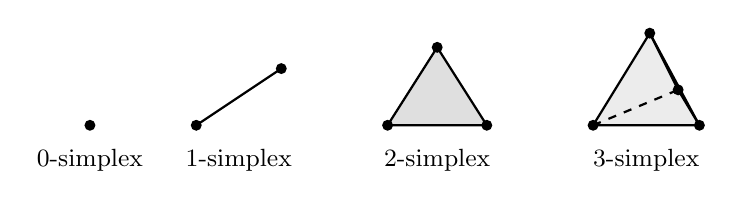
\begin{tikzpicture}[scale=0.9, v/.style={circle, fill=black, inner sep=1.4pt}]
  \node[v] at (0,0) {}; \node at (0,-0.5) {\small 0-simplex};
  \draw[thick] (1.5,0) node[v]{} -- (2.7,0.8) node[v]{}; \node at (2.1,-0.5) {\small 1-simplex};
  \fill[gray!25] (4.2,0) -- (5.6,0) -- (4.9,1.1) -- cycle;
  \draw[thick] (4.2,0) node[v]{} -- (5.6,0) node[v]{} -- (4.9,1.1) node[v]{} -- cycle; \node at (4.9,-0.5) {\small 2-simplex};
  \fill[gray!15] (7.1,0) -- (8.6,0) -- (7.9,1.3) -- cycle; \fill[gray!30] (8.6,0) -- (8.3,0.5) -- (7.9,1.3) -- cycle;
  \draw[thick] (7.1,0) node[v]{} -- (8.6,0) node[v]{} -- (7.9,1.3) node[v]{} -- cycle;
  \draw[thick] (8.6,0) -- (8.3,0.5) node[v]{} -- (7.9,1.3); \draw[thick, dashed] (7.1,0) -- (8.3,0.5);
  \node at (7.85,-0.5) {\small 3-simplex};
\end{tikzpicture}
\caption{Simplices of dimension 0 to 3.}\label{fig:simplices}
\end{figure}

\begin{definition}[Simplicial complex, {\cite{edelsbrunnerletscherzomorodian2002}}]
A \emph{simplicial complex} $K$ is a finite collection of simplices such that (i) every face of a simplex of $K$ is in $K$, and (ii) any two simplices of $K$ are disjoint or intersect in a common face.
Its \emph{vertex set} is the set of its 0-simplices.
\end{definition}

\begin{definition}[Abstract simplicial complex, {\cite{zomorodiancarlsson2005}}]
An \emph{abstract simplicial complex} on a vertex set $V$ is a collection $S$ of finite nonempty subsets of $V$ such that $\{v\} \in S$ for every $v \in V$, and $\tau \subseteq \sigma \in S$ implies $\tau \in S$.
A $k$-simplex is a set of $k+1$ vertices. Placing the vertices in general position gives a geometric realization $|S|$.
\end{definition}
The abstract version records only which vertices span simplices, and it is the form in which nerves and Mapper graphs arise below.
We write $[v_0, \dots, v_n]$ for a geometric simplex and $\{v_0, \dots, v_n\}$ for an abstract one.

\subsection{Skeleta and graphs}
\begin{definition}[Skeleton, {\cite{edelsbrunnerharerpatel2008}}]
The \emph{$k$-skeleton} $K^{(k)}$ of a simplicial complex $K$ is the subcomplex of all simplices of dimension at most $k$. The 0-skeleton is the vertex set.
\end{definition}
By the abstract definition, a finite graph $G = (V, E)$ \emph{is} a simplicial complex of dimension at most one, with its vertices as 0-simplices and its edges as 1-simplices.
Its realization $|G|$, the graph viewed as a topological space, is a \emph{topological graph}.

\begin{example}\label{ex:graph}
Let $G$ have vertices $\{a,b,c,d\}$ and edges $\{a,b\}, \{b,c\}, \{a,c\}, \{c,d\}$, and let $K = G \cup \{\{a,b,c\}\}$ add the triangle on $a,b,c$.
Then $K^{(1)} = G$.
The graph $G$ has one loop, $a \to b \to c \to a$, and in $K$ the triangle fills it.
A graph can therefore show a loop that the complex it came from does not have, which is exactly what happens in Section~\ref{sec:loops}.
\end{example}

\subsection{Nerves}
\begin{definition}[Nerve, {\cite{singh2007mapper,hatcher2001}}]
Let $\mathcal U = \{U_\alpha\}_{\alpha \in A}$ be a finite cover of a space $X$ by nonempty sets.
The \emph{nerve} $N(\mathcal U)$ is the abstract simplicial complex with vertex set $A$ in which a set $\{\alpha_0, \dots, \alpha_k\} \subseteq A$ spans a $k$-simplex if and only if $U_{\alpha_0} \cap \cdots \cap U_{\alpha_k} \neq \emptyset$.
\end{definition}

\begin{example}\label{ex:nerve}
Cover a circle by three arcs, each overlapping the next, with no point in all three.
The nerve has three vertices and three edges but no triangle, so it is a hollow triangle, homotopy equivalent to the circle.
Cover a disk instead by three disks that share a common point. The nerve is then a filled triangle, homotopy equivalent to a point, and so to the disk (Figure~\ref{fig:nerve}).
\end{example}

\begin{figure}[htbp]
\centering
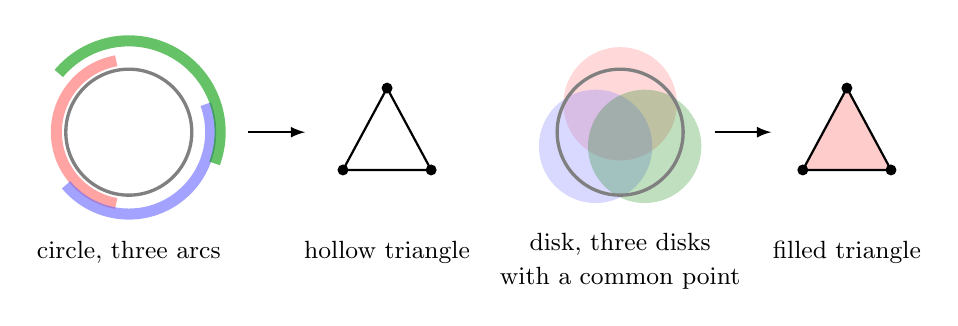
\begin{tikzpicture}[scale=0.8, v/.style={circle, fill=black, inner sep=1.4pt}]
  \draw[very thick, gray] (0,0) circle (1);
  \draw[line width=4pt, red!60, opacity=0.6] (100:1.15) arc (100:260:1.15);
  \draw[line width=4pt, blue!60, opacity=0.6] (220:1.3) arc (220:380:1.3);
  \draw[line width=4pt, green!60!black, opacity=0.6] (340:1.45) arc (340:500:1.45);
  \node at (0,-1.9) {\small circle, three arcs};
  \draw[-latex, thick] (1.9,0) -- (2.8,0);
  \draw[thick] (3.4,-0.6) node[v]{} -- (4.8,-0.6) node[v]{} -- (4.1,0.7) node[v]{} -- cycle;
  \node at (4.1,-1.9) {\small hollow triangle};
  \begin{scope}[xshift=7.8cm]
  % three disks of radius 0.9 centred 0.45 from the origin: together they cover the unit disk, and all contain the origin
  \fill[red!50, opacity=0.3] (90:0.45) circle (0.9); \fill[blue!50, opacity=0.3] (210:0.45) circle (0.9); \fill[green!50!black, opacity=0.25] (330:0.45) circle (0.9);
  \draw[very thick, gray] (0,0) circle (1);
  \node[align=center] at (0,-2.05) {\small disk, three disks\\\small with a common point};
  \draw[-latex, thick] (1.5,0) -- (2.4,0);
  \fill[red!20] (2.9,-0.6) -- (4.3,-0.6) -- (3.6,0.7) -- cycle;
  \draw[thick] (2.9,-0.6) node[v]{} -- (4.3,-0.6) node[v]{} -- (3.6,0.7) node[v]{} -- cycle;
  \node at (3.6,-1.9) {\small filled triangle};
  \end{scope}
\end{tikzpicture}
\caption{Two covers and their nerves (Example~\ref{ex:nerve}).}\label{fig:nerve}
\end{figure}

\subsection{The nerve theorem}
In both examples the nerve has the shape of the space. The nerve theorem gives conditions under which this holds.
A set $C \subseteq \R^d$ is \emph{convex} if the segment between any two points of $C$ lies in $C$.

\begin{theorem}[Nerve theorem, closed convex version, {\cite[Thm.~3.9]{bauerkerberrollrolle2023}}]\label{thm:nerve}
If $X \subseteq \R^d$ is the union of finitely many closed convex sets $\mathcal C = \{C_1, \dots, C_n\}$, then $X \simeq |N(\mathcal C)|$.
\end{theorem}
An early closed-cover version is due to \textcite[Cor.~3]{borsuk1948}.
The idea behind the hypothesis is that a nonempty intersection of convex sets is convex, hence contractible, so each simplex of the nerve stands for a contractible piece of $X$.
There is also an open-cover version. If $\mathcal U$ is an open cover of a paracompact space $X$ and every nonempty finite intersection of its sets is contractible, then $X \simeq |N(\mathcal U)|$ \parencite{hatcher2001}.

\begin{remark}
Covers built from data are rarely this well behaved. The sets Mapper produces are clusters, which need not be convex, and their intersections need not be contractible. A Mapper graph therefore need not have the shape of the underlying space, and this is why Sections~\ref{sec:certify} and~\ref{sec:shape} test its features before we trust them.
\end{remark}

\subsection{Homology and Betti numbers}
\begin{definition}[Betti numbers, {\cite{hatcher2001}}]
The $k$-th \emph{Betti number} $b_k(X)$ is the rank of the $k$-th homology group $H_k(X)$. We use coefficients in $\Z_2$, so each $H_k$ is a vector space and $b_k$ is its dimension.
\end{definition}
The number $b_0$ counts path components \parencite{hatcher2001}, and $b_1$ counts independent loops.
For the complexes in this paper both are computable by linear algebra over $\Z_2$.
For a simplicial complex $K$, let $C_k$ be the $\Z_2$-vector space with basis the $k$-simplices, and let $\partial_k : C_k \to C_{k-1}$ send each simplex to the sum of its $(k-1)$-dimensional faces. Then $H_k(K) = \ker \partial_k / \operatorname{im} \partial_{k+1}$.

For a finite graph $G$ with $V$ vertices, $E$ edges, and $C$ connected components, the Euler characteristic gives $V - E = b_0 - b_1$ with $b_0 = C$, so
\begin{equation}\label{eq:graph-b1}
  b_1(G) = E - V + C.
\end{equation}
In a complex of dimension two, triangles can fill loops, and
\begin{equation}\label{eq:complex-b1}
  b_1(K) = E - V + C - \rank \partial_2,
\end{equation}
where $\partial_2$ maps each triangle to its three edges.
A hollow triangle has $b_1 = 3 - 3 + 1 = 1$, and filling it gives $\rank \partial_2 = 1$ and $b_1 = 0$.
Equation~\eqref{eq:complex-b1} is how Section~\ref{sec:loops} computes the loops of the full nerve.

\subsection{Reeb graphs and Reeb spaces}
The construction in this subsection goes back to \textcite{reeb1946}.
\begin{definition}[Reeb graph, {\cite{carriereoudot2018,reeb1946}}]
Let $f : X \to \R$ be continuous. Write $x \sim y$ if $f(x) = f(y)$ and $x$ and $y$ lie in the same connected component of the level set $f^{-1}(f(x))$.
The \emph{Reeb graph} of $f$ is the quotient space $R_f(X) = X/{\sim}$.
\end{definition}
A smooth function $f$ on a manifold is a \emph{Morse function} if its Hessian is nondegenerate at every critical point \parencite[Def.~1.21]{debray2018morse}.
When $X$ is a compact smooth manifold and $f$ is a Morse function, or more generally of Morse type, $R_f(X)$ is a graph (technically a multigraph) and so a topological graph \parencite[p.~1334]{carriereoudot2018}.
For the height function on an upright torus, each level set collapses to one point per component, giving one point near the bottom and top and two in the middle band (Figure~\ref{fig:reeb}). The Reeb graph is a circle with two whiskers.
Replacing $\R$ by $\R^k$ and level sets by the preimages $f^{-1}(c)$, $c \in \R^k$, gives the \emph{Reeb space} \parencite{munchwang2016,edelsbrunnerharerpatel2008}.

\begin{figure}[htbp]
\centering
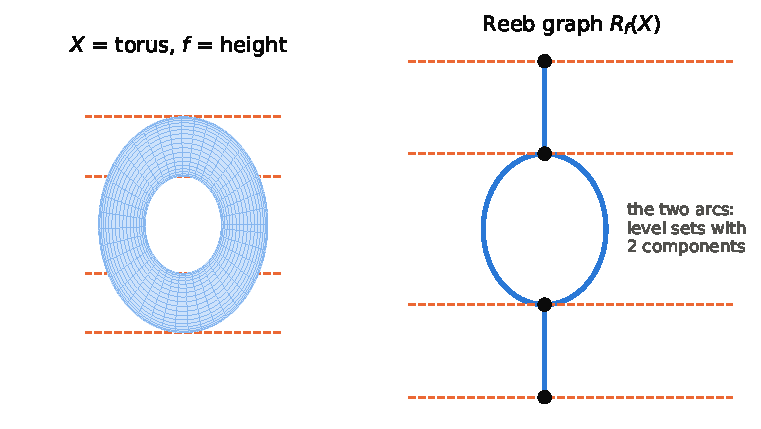
\includegraphics[width=0.62\textwidth]{reeb_torus.pdf}
\caption{The height function on a torus and its Reeb graph.}\label{fig:reeb}
\end{figure}

%======================================================================
\section{The Mapper algorithm}\label{sec:mapper}
%======================================================================
Singh, M\'emoli, and Carlsson introduced Mapper in 2007 \parencite{singh2007mapper}.
We first describe the topological version, which works on a space, and then the statistical version, which works on a finite sample and is what we run on pitch data.

\subsection{Topological Mapper}
\begin{definition}[Mapper, {\cite{singh2007mapper,deymemoliwang2017}}]
Let $f : X \to Z$ be continuous and let $\mathcal U = \{U_\alpha\}$ be a finite open cover of $Z$.
Split each preimage $f^{-1}(U_\alpha)$ into its path components. Together they form the \emph{pullback cover} $f^*\mathcal U$ of $X$.
The \emph{Mapper} is its nerve, $M(\mathcal U, f) = N(f^*\mathcal U)$.
\end{definition}
For $Z = \R$, Mapper is a discrete estimator of the Reeb graph, and for $Z = \R^d$ it approximates the Reeb space \parencite{carrieremicheloudot2018,munchwang2016}.
Dey, M\'emoli, and Wang showed that the loops of a Mapper are controlled by those of $X$.

\begin{theorem}[Dey--M\'emoli--Wang, {\cite{deymemoliwang2017}}]\label{thm:dmw}
If $\mathcal U$ is a finite open cover of a compact space $X$ by path-connected sets, the nerve map induces a surjection $H_1(X) \to H_1(N(\mathcal U))$, with $\Z_2$ coefficients.
\end{theorem}
When $f$ is well behaved, so that each preimage $f^{-1}(U_\alpha)$ has finitely many path components and they are open, the pullback cover is such a cover \parencite{deymemoliwang2017}, and therefore
\begin{equation}\label{eq:mapper-b1}
  b_1(M(\mathcal U, f)) \le b_1(X).
\end{equation}
This bound concerns the nerve, a simplicial complex. Software outputs only its 1-skeleton, whose loops are not bounded this way (Example~\ref{ex:graph}), and Section~\ref{sec:loops} shows the difference in our data.

\subsection{Statistical Mapper}
A \emph{point cloud} is a finite set $P \subseteq \R^n$ with Euclidean distance.
In the statistical version of Mapper, clustering plays the role of path components, and each preimage $f^{-1}(U_\alpha) \cap P$ is split into clusters \parencite{singh2007mapper}.
The algorithm has four steps:
\begin{enumerate}
  \item choose a \emph{lens} $f : P \to \R^k$;
  \item cover $f(P)$ by overlapping sets;
  \item cluster each preimage, in the full space $\R^n$;
  \item form the \emph{Mapper graph}, with one vertex per cluster and one edge for each pair of clusters that share a point.
\end{enumerate}
Steps 1--3 build a cover of $P$ and step 4 takes its nerve \parencite{singh2007mapper}, keeping only the 1-skeleton.
The lens decides which points are clustered at the same time, since only points in the same preimage are clustered together, while the clustering itself uses all $n$ coordinates.

\begin{example}\label{ex:toy}
We follow one example through the rest of this section and the next.
Take the 240 noisy points $P$ on a circle of radius 1 shown in Figure~\ref{fig:toy}.
Its lens will be one-dimensional and its cover a set of intervals, whereas our real analysis uses a two-dimensional lens and squares, but each step works the same way.
The subsections below build Mapper on this circle one step at a time.
\end{example}

\begin{figure}[htbp]
\centering
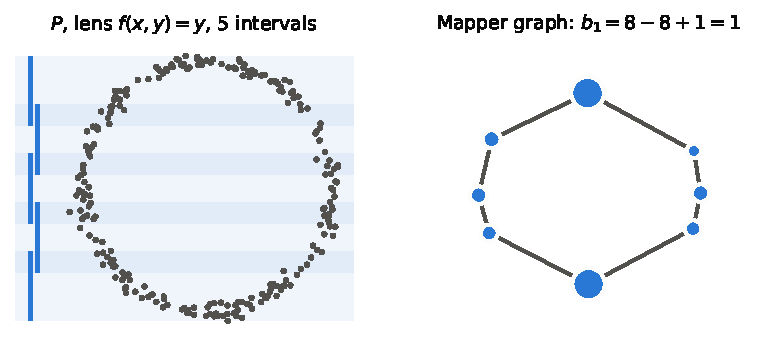
\includegraphics[width=0.75\textwidth]{toy_mapper.pdf}
\caption{Mapper on a noisy circle (Example~\ref{ex:toy}). Left, the 240 points and the five intervals of the cover. Right, the resulting graph.}\label{fig:toy}
\end{figure}

\subsection{The lens: principal component analysis}
Principal component analysis (PCA) goes back to \textcite{pearson1901}.
It finds new uncorrelated variables, linear combinations of the old ones, that successively capture as much variance as possible \parencite{jolliffecadima2016,pearson1901}.
Among the Mapper applications reviewed by \textcite{madukpe2026review}, PCA is the most commonly used lens, and we use a two-dimensional PCA lens.

Let the data be $m$ observations of $n$ features, and subtract each column's mean to obtain the centered matrix $\mathbf A \in \R^{m \times n}$.
We center the data because variance is measured around the mean.
Centering therefore changes neither the covariance matrix nor the principal components, and afterward the covariance matrix is $S = \frac{1}{m-1}\mathbf A^{\mathsf T}\mathbf A$, so we can read the principal components directly from $\mathbf A$ \parencite{jolliffecadima2016}.
The diagonal entries of $S$ are the feature variances and its off-diagonal entries the covariances.

Since $S^{\mathsf T} = S$, the spectral theorem gives $S$ real eigenvalues and an orthonormal basis of eigenvectors.
Since $x^{\mathsf T} S x = \frac{1}{m-1}\|\mathbf A x\|^2 \ge 0$ for every $x \in \R^n$, the eigenvalues are also nonnegative.
The variance of the data along a unit vector $v$ is $v^{\mathsf T} S v$, which is maximized by a top eigenvector.

\begin{theorem}[Singular value decomposition, {\cite{axler2024ladr}}]
Let $\mathbf A$ have rank $r \ge 1$. Then $\mathbf A = \mathbf U \boldsymbol\Sigma \mathbf V^{\mathsf T}$, where $\mathbf U \in \R^{m \times r}$ and $\mathbf V \in \R^{n \times r}$ have orthonormal columns and $\boldsymbol\Sigma = \operatorname{diag}(\sigma_1 \ge \cdots \ge \sigma_r > 0)$.
\end{theorem}
The columns of $\mathbf V$ are eigenvectors of $\mathbf A^{\mathsf T}\mathbf A$, and the columns of $\mathbf U$ eigenvectors of $\mathbf A\mathbf A^{\mathsf T}$, for the nonzero eigenvalues $\sigma_i^2$. Hence the eigenvalues of $S$ are $\lambda_i = \sigma_i^2/(m-1)$ and the principal directions are the columns $v_i$ of $\mathbf V$ \parencite{jolliffecadima2016}.
Keeping the first $k$ directions, $\mathbf V_k = [v_1 \cdots v_k]$, the lens is $f(x) = \mathbf V_k^{\mathsf T} (x - \bar x)$, where $\bar x$ is the mean, and the score matrix is $\mathbf Z_k = \mathbf A \mathbf V_k = \mathbf U_k \boldsymbol\Sigma_k$.
The matrix $\mathbf A_k = \mathbf U_k \boldsymbol\Sigma_k \mathbf V_k^{\mathsf T}$ is the closest matrix of rank at most $k$ to $\mathbf A$, both in the operator norm, with error $\sigma_{k+1}$ \parencite{axler2024ladr}, and in the least-squares sense \parencite{jolliffecadima2016}.
The proportion of variance explained by component $j$ is $\lambda_j / \sum_l \lambda_l = \sigma_j^2 / \sum_l \sigma_l^2$ \parencite{jolliffecadima2016}.

We take $k = 2$.
The cover lives in $\R^k$, and with ten intervals per axis, $k = 2$ gives 100 cubes, while $k = 3$ would give 1{,}000, most of them nearly empty. A two-dimensional lens also has the advantage that we can draw it and read it.
Because PCA is linear, it can flatten curved structure. We accept this because clustering happens in the full space, and Section~\ref{sec:certify} repeats the stability analysis with three other lenses, including the nonlinear Isomap \parencite{tenenbaum2000isomap}.

For the circle of Example~\ref{ex:toy}, the variance is nearly the same in every direction, so the first principal direction is not well determined.
We choose the vertical direction, which gives the height $f(x,y) = y$ as the lens.

\subsection{The cover}
The image $f(P) \subseteq \R^k$ is covered by overlapping hypercubes. Each axis is cut into intervals that overlap their neighbors by a fixed percentage \parencite{singh2007mapper,madukpe2026review}.
Two parameters set the resolution, the number of intervals and the percentage overlap \parencite{singh2007mapper}. The resulting graph depends on them, and tuning them on real data is not easy \parencite{carrieremicheloudot2018}.
We use ten intervals per axis with 30\% overlap and test the results over a grid of alternatives (Section~\ref{sec:certify}).
For the circle, we cover the range of heights by five intervals with 30\% overlap. Because the overlap is less than 50\%, no height lies in three intervals at once.

\subsection{Clustering: DBSCAN}\label{sec:dbscan}
DBSCAN was introduced by \textcite{ester1996dbscan} in 1996, and it is the second most common choice in reviewed Mapper applications after hierarchical clustering \parencite{madukpe2026review}.
It needs no preset number of clusters, finds clusters of arbitrary shape, and labels isolated points as noise \parencite{ester1996dbscan}.
Fix a point cloud $P$ with distance $d$, a radius $\varepsilon > 0$, and a count $M \in \N$ (called Eps and MinPts by \textcite{ester1996dbscan}). The following definitions are theirs.

\begin{definition}
The \emph{$\varepsilon$-neighborhood} of $p \in P$ is $N_\varepsilon(p) = \{ q \in P : d(p,q) \le \varepsilon \}$, and $p$ is a \emph{core point} if $\# N_\varepsilon(p) \ge M$.
A point $p$ is \emph{directly density-reachable} from $q$ if $p \in N_\varepsilon(q)$ and $q$ is a core point, and \emph{density-reachable} from $q$ if there is a chain $q = p_1, p_2, \dots, p_k = p$ in which each $p_{i+1}$ is directly density-reachable from $p_i$.
Points $p$ and $q$ are \emph{density-connected} if both are density-reachable from some common point $o$.
\end{definition}
\begin{definition}
A \emph{cluster} is a nonempty $C \subseteq P$ such that (i) if $p \in C$ and $q$ is density-reachable from $p$, then $q \in C$ (maximality), and (ii) any two points of $C$ are density-connected (connectivity).
\emph{Noise} is the set of points of $P$ in no cluster, so it depends on the chosen $(\varepsilon, M)$.
\end{definition}
\begin{lemma}[{\textcite{ester1996dbscan}}]
If $C$ is a cluster and $p \in C$ is a core point, then $C = \{ o \in P : o \text{ is density-reachable from } p \}$.
\end{lemma}
The algorithm loops over the points and expands a new cluster from each unclassified core point \parencite[p.~229]{ester1996dbscan}. A point that is not a core point is marked noise for now, and a border point first marked noise is relabeled if a later cluster reaches it.
The lemma is why this is correct. A cluster is determined by any one of its core points, so starting from an unclassified core point and collecting everything density-reachable from it recovers exactly its cluster.
Although \textcite{ester1996dbscan} allow separate parameters for each cluster, their algorithm uses a single pair, and so do we, with $\varepsilon = 1.0$ in standardized units and $M = 4$.
Figure~\ref{fig:dbscan} illustrates the three kinds of point on a separate small example.

For the circle we use $\varepsilon = 0.25$ and $M = 3$.
DBSCAN then splits the five preimages into $1, 2, 2, 2, 1$ arcs, since the top and bottom intervals each meet the circle in one arc and the middle three meet it in two.

\begin{figure}[htbp]
\centering
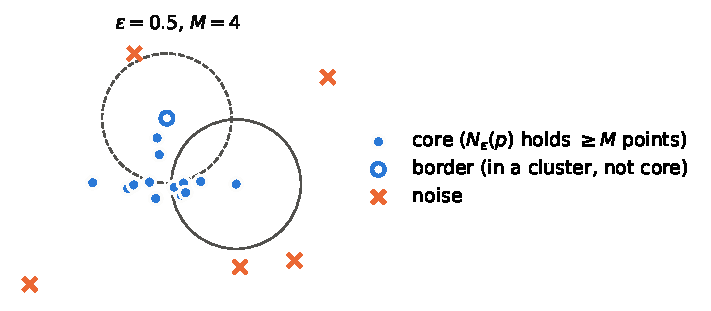
\includegraphics[width=0.6\textwidth]{dbscan_toy.pdf}
\caption{A separate illustration of core, border, and noise points, for $\varepsilon = 0.5$ and $M = 4$. Solid circle, a core point's $\varepsilon$-ball, which holds six points. Dashed circle, a border point's ball, which holds three points including a core point, so the border point joins the cluster. Crosses, noise points, each more than $\varepsilon$ from every core point.}\label{fig:dbscan}
\end{figure}

\subsection{The graph and its implementation}
Each cluster becomes a vertex, and two clusters are joined by an edge when they share at least one point, which happens because neighboring cubes overlap \parencite{singh2007mapper}.
The clusters form a cover of the non-noise part of $P$, and the graph is the 1-skeleton of its nerve. Three clusters with a common point span a triangle in the nerve, but the graph keeps only the three edges.
We use KeplerMapper, a Python implementation that works with scikit-learn-compatible clustering and scaling algorithms \parencite{vanveen2019keplermapper,pedregosa2011sklearn}, developed under the scikit-tda project \parencite{keplermapper_repo}.

For the circle, no point lies in three intervals, so no three clusters share a point.
The graph has 8 vertices and 8 edges in one component, so by~\eqref{eq:graph-b1} it has $b_1 = 8 - 8 + 1 = 1$, and since there are no triangles, the nerve is the graph.
Mapper has recovered the single loop of the circle, which is also the circle's Reeb graph for the height function.

%======================================================================
\section{Data collection}\label{sec:data}
%======================================================================
We downloaded Statcast pitch-tracking data \parencite{savantcsvdocs} with pybaseball \parencite{ledoux_pybaseball}.
The main analysis uses the 2025 regular season and postseason, \NPitches{} pitches.
We describe each pitch by eight of the measurements in Section~\ref{sec:statcast}: release speed, $\mathit{pfx}_x$, $\mathit{pfx}_z$, spin rate, spin axis, extension, and the horizontal and vertical release position.

Left-handed pitchers are mirrored into the right-handed frame, so $\mathit{pfx}_x$ and the horizontal release position change sign and the spin axis $\theta$ becomes $360^\circ - \theta$.
The spin axis is an angle, so $\theta$ and $\theta + 360^\circ$ are the same direction. We therefore encode it as the point $(\cos\theta, \sin\theta)$ on the circle instead of as a number in $[0, 360)$, which gives nine coordinates in all.

The unit of analysis is a \emph{pitch shape}, the average of one pitcher's pitches of one type.
Averaging removes pitch-to-pitch noise and keeps each pitcher's stable profile, and it gives \NShapes{} shapes in $\R^{\NFeatures}$, which we standardize to mean zero and unit variance.
We applied no minimum pitch count in the fit. The median shape averages \MedianPitches{} pitches, but \PctLtFive\% average fewer than five and \PctLtTwenty\% fewer than twenty. The \NSlow{} slow shapes (below 70 mph) are the thinnest, with a median of \SlowMedian{} pitches and a quarter at \SlowQ{} or fewer.
Appendix~\ref{app:thin} repeats the main Mapper fit with minimum counts of 10 and 20.
Statcast revises some pitch labels after the fact, so rebuilding the shapes from a later download gives counts that differ by a few (\SSOneShapes{} instead of \NShapes).

Some analyses use a smaller set of coordinates that we call \emph{flight space}.
It consists of velocity relative to the pitcher's fastest pitch shape, $\mathit{pfx}_x$, $\mathit{pfx}_z$, spin rate, and the spin axis, six coordinates in all.
Flight space leaves out the delivery (release position and extension) and absolute velocity, which make a pitcher's own pitches look alike.
The density-peak analysis (Section~\ref{sec:peaks}) works with single pitches and uses a related coordinate, speed relative to the pitcher's 95th-percentile speed in that game.

We use the 2026 season (\NPitchesTwentySix{} pitches) to replicate the evaluation result in Section~\ref{sec:consequences}.

%======================================================================
\section{Certifying the Mapper picture}\label{sec:certify}
%======================================================================
Although a Mapper graph gives a useful picture, the picture alone does not tell us which of its features are real.
To test a feature, we asked whether it survives reasonable changes to the construction and whether a null model without that structure also produces it.
We then computed the homology of the full nerve, along with invariants that do not depend on Mapper whatsoever, namely persistent homology, intrinsic dimension, and density peaks.

Others have raised the same concern about Mapper.
\textcite{carrieremicheloudot2018} show that Mapper's output depends strongly on the cover parameters, and they develop a statistical analysis and a principled parameter selection. We use a parameter grid and resampling instead, and we see their approach as an alternative.
\textcite{vejdemojohansson2018certified} note that Mapper does not check whether its cover meets the requirements of the nerve lemma, and they propose statistical tests for obstructions.
\textcite{topaz2026null} shows that the covariance structure of data alone can make Mapper communities look differentiated, proposes a Gaussian null model with the sample covariance, and finds that four published Mapper analyses do not exceed it at the 0.05 level once singleton communities are set aside. Topaz notes that a non-rejection does not rule out subtypes and that the proof is given in an idealized setting.
We arrived at the same covariance-matched null independently, designing our comparisons in the spirit of hypothesis testing for persistent homology \parencite{robinsonturner2017,blumberg2014}, and we apply it beyond communities, to the graph's features, its loops, the homology of the point cloud, its intrinsic dimension, and its density peaks.

\subsection{Stability}
We refit the graph over a 27-point grid, with 8, 10, or 12 intervals per axis, 20, 30, or 40\% overlap, and $\varepsilon = 0.8$, 1.0, or 1.2.
We also refit it 30 times on a random 80\% of pitchers drawn without replacement.
We repeat every fit with four lenses, namely the PCA lens, velocity against induced vertical break, a two-dimensional Isomap embedding, and a one-dimensional density lens given by the mean distance to the ten nearest neighbors.

Node labels change between fits, so we define features by their content.
\emph{Connectivity} is the number of components and the size of the largest.
\emph{Slow-pitch isolation} asks whether most shapes slower than 70 mph lie outside the largest component.
We measure it only in fits where the slow shapes form a node of their own.
For the \emph{velocity ordering}, we take the node of the largest component with the highest share of curveballs and the node with the highest share of four-seam fastballs, among nodes above a minimum size. We then compute Spearman's $\rho$ between node velocity and position along the shortest path between them, and we count the ordering as present when $\rho \ge 0.7$.

\subsection{Null models}
We refit each null through the identical pipeline.
The \emph{Gaussian null} has the same mean and covariance as the shapes and no structure beyond these second moments.
The \emph{within-type shuffle} permutes each feature independently among shapes of the same pitch type, which keeps each type's marginal distributions but destroys the joint structure inside it.
The \emph{spin-pair shuffle} does the same but permutes $(\cos\theta, \sin\theta)$ together, so that shuffled shapes still have a valid spin axis.
A feature counts as evidence of structure only if real fits show it clearly more often than null fits.

\subsection{Loops of the full nerve}
For each fit we compute the first Betti number of the graph by~\eqref{eq:graph-b1} and of the full nerve by~\eqref{eq:complex-b1}, adding a triangle for every three clusters with a common point and computing $\rank \partial_2$ over $\Z_2$.
We read the loops of a nerve by comparing them with the null models. This step is our own design and does not follow from~\eqref{eq:mapper-b1}. If a null model also produces nerve loops, we do not count them as evidence of loops in the data.

\subsection{Persistent homology}
Persistent homology was developed by \textcite{edelsbrunnerletscherzomorodian2002} and \textcite{zomorodiancarlsson2005}.
For a finite metric space $(P, d)$ and scale $t \in \R$, the Vietoris--Rips complex is $\mathrm{Rips}_t(P) = \{ \emptyset \neq S \subseteq P : \diam S \le t \}$ \parencite{bauer2021ripser}.
As $t$ grows these complexes are nested, and persistent homology records the scale at which each component or loop is born and dies \parencite{edelsbrunnerletscherzomorodian2002,zomorodiancarlsson2005}.
An $H_0$ bar that lives long is a gap between groups of points, and a long $H_1$ bar is a loop.
We compute persistence with Ripser \parencite{bauer2021ripser,tralie2018ripserpy} on five random subsamples of 1{,}000 standardized shapes, for the real data and the nulls.

Points far from the diagonal of a persistence diagram are usually read as features and points near it as noise \parencite{fasy2014confidence}.
We do not compute formal confidence sets. Instead we compare with the nulls, measuring persistence in units of the median $H_0$ death of the real data.
We count an $H_0$ bar as long-lived if it dies after 3 units and an $H_1$ loop as persistent if its persistence exceeds 2 units. These cutoffs are our convention for the pitch data.

Figure~\ref{fig:rips} shows a persistent loop on a separate 40-point sample of a noisy circle, measured in raw distance.
One loop is born at scale 0.625 and dies at 1.617, a persistence of 0.992, while the next-longest loop has persistence 0.005.

\begin{figure}[htbp]
\centering
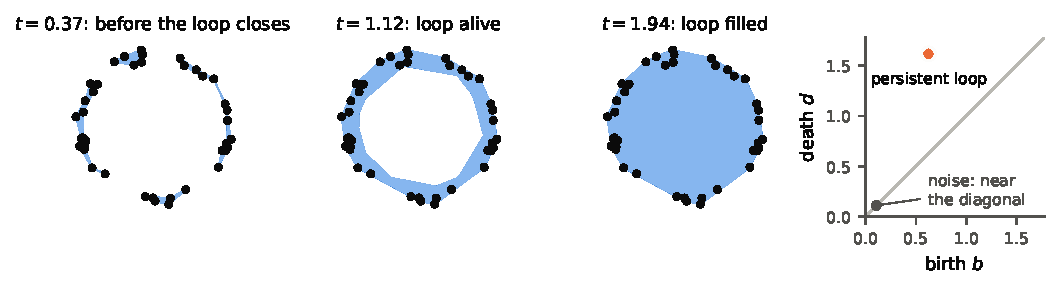
\includegraphics[width=\textwidth]{rips_toy.pdf}
\caption{A persistent loop. Rips complexes of a noisy circle at three scales (before the loop closes, while it is alive, and after it is filled) and the $H_1$ persistence diagram, in which the loop is the one point far from the diagonal.}\label{fig:rips}
\end{figure}

\subsection{Intrinsic dimension}
We estimate the dimension of the point cloud with the maximum-likelihood estimator of \textcite{levinabickel2004}, using ten neighbors and the averaging of \textcite{mackay2005comments}, and with TwoNN \parencite{facco2017twonn}.
Both use nearest-neighbor distances.
We compare with the spin-pair shuffle, which keeps each type's marginals and the spin-axis constraint, both overall and within each pitch type.

\subsection{Density peaks}\label{sec:peaks}
Vietoris--Rips persistence detects gaps, but it cannot tell a space with one dense region from one with several.
To look for dense regions, we follow \textcite{maloof2026classify} and compute the persistence of the superlevel sets of a smoothed density at the pitch level.
We use speed relative to the pitcher's 95th-percentile speed in that game, horizontal break, and induced vertical break, on a $50^3$ grid (horizontal and vertical break from $-25$ to 25 inches, relative speed from $-25$ to 5 mph), smoothed by a Gaussian of one grid cell.
We compare each peak's persistence with the largest secondary peak in 50 covariance-matched Gaussian replicates, which gives a Monte Carlo $p$-value.
A Gaussian has one peak, so this test only shows that there is more than one. We judge small peaks by their robustness to the smoothing (1, 1.5, and 2 cells) and to random halves of the data.
We repeat the analysis in one dimension, for the pitch shapes along the first principal component.

\subsection{Review of the running example}
Table~\ref{tab:review} collects what each step gives on the noisy circle, together with the same steps run on five Gaussian samples with the circle's mean and covariance.
The circle has one loop, and every step that should see it does.

\begin{table}[htbp]
\centering
\begin{tabular}{lll}
\toprule
Step & Noisy circle & Gaussian null (5 samples) \\
\midrule
Lens & height $f(x,y) = y$ & same \\
Cover & 5 intervals, 30\% overlap & same \\
Clustering & DBSCAN ($\varepsilon = 0.25$, $M = 3$): $1, 2, 2, 2, 1$ arcs & same settings \\
Mapper graph & 8 vertices, 8 edges, $b_1 = 1$ & $b_1 = \CircNullGraphBoneMax$, \CircNullCompLo--\CircNullCompHi{} components \\
Full nerve & no triangles, $b_1 = 1$ & no triangles \\
\bottomrule
\end{tabular}
\caption{The running example, step by step, against a same-covariance Gaussian null.}\label{tab:review}
\end{table}

Since the clusters here are arcs of a finite sample, the bound~\eqref{eq:mapper-b1} is a guide for this example and not a theorem about it. Its prediction, at most one loop, still holds.

%======================================================================
\section{The shape of pitch space}\label{sec:shape}
%======================================================================
We now apply these methods to the 2025 pitch shapes. We first describe the Mapper graph and then ask which of its features survive the tests of Section~\ref{sec:certify}.

The first two principal components explain \PCone\% and \PCtwo\% of the variance.
The first separates fastballs from breaking balls. The second is mostly delivery (extension and release height) together with velocity, and the very slow pitches sit at its bottom (Figure~\ref{fig:lens}).
The Mapper graph (Figure~\ref{fig:graph}) has \NNodes{} nodes, \NEdges{} edges, and \NComponents{} components.
One giant component runs from curveballs through sliders and cutters to fastballs and changeups, ordered by velocity, while the very slow pitches (eephus pitches and position players pitching) sit apart.

\begin{figure}[htbp]
\centering
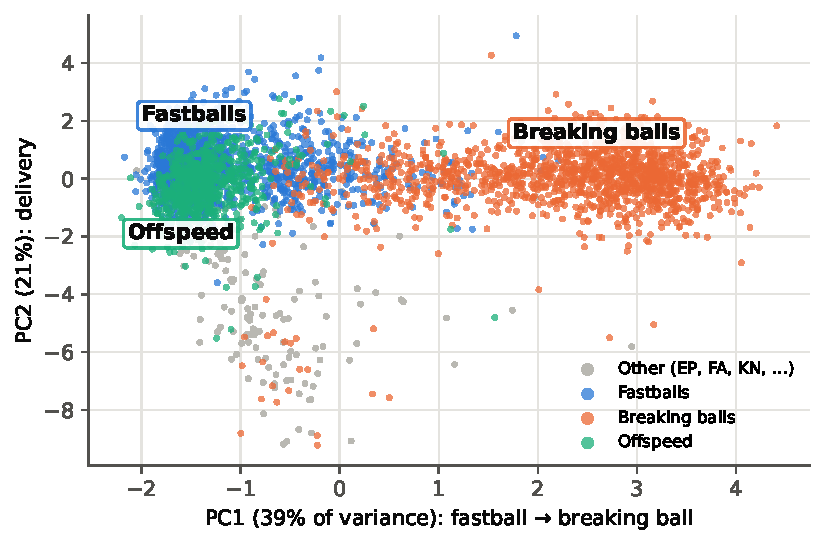
\includegraphics[width=0.7\textwidth]{lens_scatter.pdf}
\caption{The 2025 pitch shapes in the PCA lens, by pitch family.}\label{fig:lens}
\end{figure}

\begin{figure}[htbp]
\centering
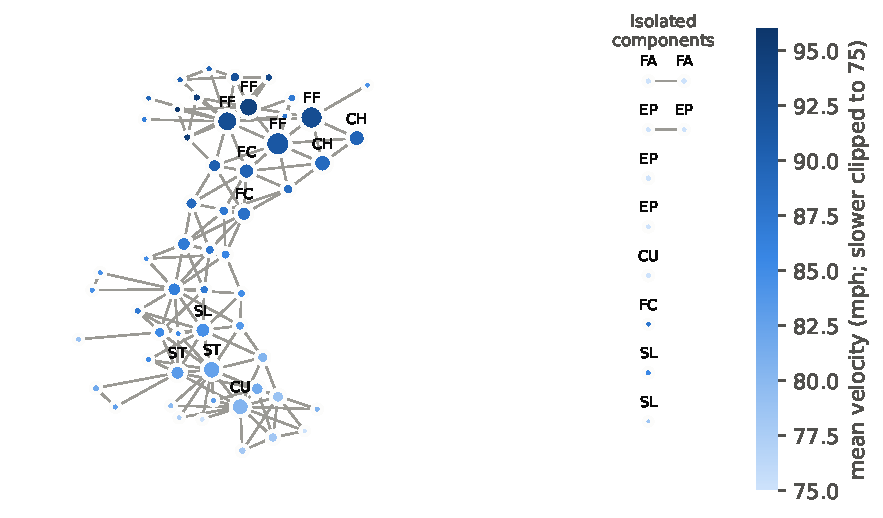
\includegraphics[width=0.75\textwidth]{mapper_graph.pdf}
\caption{The Mapper graph, nodes colored by mean velocity.}\label{fig:graph}
\end{figure}

Both features are stable (Table~\ref{tab:stability}).
The velocity ordering holds in \StabOrderMin\% of fits under every lens, and slow-pitch isolation in \StabSlowPCALo--\StabSlowPCAHi\% of fits with the PCA lens and \StabSlowLo--\StabSlowHi\% across lenses.
However, the null models also reproduce both features. The velocity ordering appears in \NullOrderMin\% of null fits, which tells us it reflects the covariance of the features and not hidden topology.
Slow-pitch isolation appears in \NullSlowLo--\NullSlowHi\% of null fits, so it is only somewhat stronger in the real data than the nulls produce.
A third feature, a ``bridge'' of sliders and cutters with the highest betweenness centrality, looked interesting in the PCA graph. It changed when we changed the lens and was reproduced by the nulls, so we do not report it as a finding.

\begin{table}[htbp]
\centering
\begin{tabular}{lcc}
\toprule
Feature (share of fits) & Real data & Null models \\
\midrule
Velocity ordering ($\rho \ge 0.7$) & \StabOrderMin\% (every lens) & \NullOrderMin\% \\
Slow shapes isolated & \StabSlowLo--\StabSlowHi\% & \NullSlowLo--\NullSlowHi\% \\
\bottomrule
\end{tabular}
\caption{Stability across the parameter grid, subsamples of pitchers, and four lenses, against the Gaussian and within-type-shuffle nulls. Slow-pitch isolation is measured only in fits where the slow shapes form a node of their own.}\label{tab:stability}
\end{table}

\subsection{Loops are artifacts of the 1-skeleton}\label{sec:loops}
By~\eqref{eq:graph-b1} the graph has $b_1 = \NEdges - \NNodes + \NComponents = \GraphBone$ independent cycles.
The full nerve adds a triangle for every three clusters with a common point. Its boundary map $\partial_2$ has rank \NerveRank{} over $\Z_2$, so by~\eqref{eq:complex-b1} the nerve has $b_1 = \GraphBone - \NerveRank = \NerveBone$.
Across the 27 parameter choices the graph has between \GridGraphBoneMin{} and \GridGraphBoneMax{} loops, while the nerve has between \GridNerveBoneMin{} and \GridNerveBoneMax.
The null models show the same pattern of many graph loops and few nerve loops. Gaussian graphs have \GaussGraphBoneMin--\GaussGraphBoneMax{} loops and their nerves \GaussNerveBoneMin--\GaussNerveBoneMax, and within-type shuffle graphs have \ShuffleGraphBoneMin--\ShuffleGraphBoneMax{} and their nerves \ShuffleNerveBoneMin--\ShuffleNerveBoneMax.
The graph's loops come from reading only the 1-skeleton (Example~\ref{ex:graph}), and the nerve's triangles fill them.

We should be careful about how far Theorem~\ref{thm:dmw} reaches.
It concerns a cover of a space by path-connected sets, while our cover is made of DBSCAN clusters, which are not path components, built on a finite sample.
So the theorem does not strictly apply, and a nerve can keep a few loops, as ours do (\GridNerveBoneMin--\GridNerveBoneMax) and as the nulls' do (\NullNerveBoneMin--\NullNerveBoneMax).
With that caveat, persistent homology of the shapes finds no persistent loops (Figure~\ref{fig:persistence}), so the data appear to have no loops, and if the theorem applied, no Mapper nerve of them could have loops either.
The theorem and the evidence point the same way, but together they fall short of a proof about the data.

\begin{figure}[htbp]
\centering
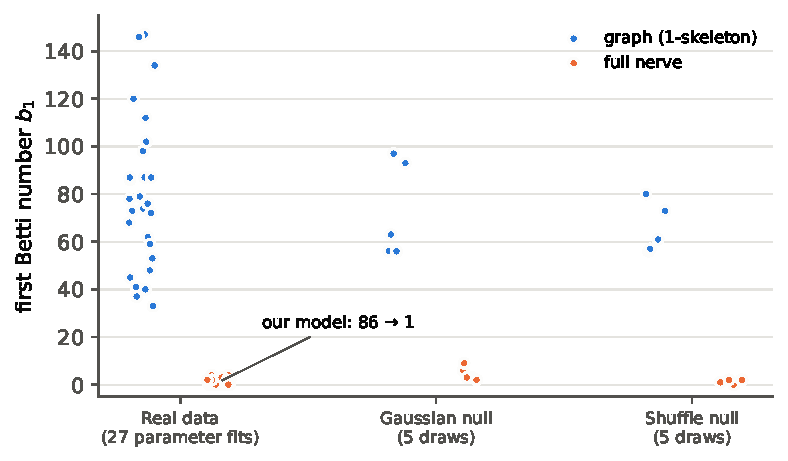
\includegraphics[width=0.7\textwidth]{nerve_b1.pdf}
\caption{First Betti number of the Mapper graph and of the full nerve, for real fits and null models.}\label{fig:nerveb1}
\end{figure}

\subsection{Gaps, dimension, and dense regions}
Next, we checked whether the space has gaps.
On subsamples of 1{,}000 shapes, the real data have \PHRealLongBars{} long-lived $H_0$ bars and the Gaussian null has \PHGaussLongBarsLo{} to \PHGaussLongBarsHi, so the data have no more gaps than a Gaussian with the same covariance. They are also more concentrated, with a median $H_0$ death of \PHRealHzeroMedian{} against \PHGaussHzeroMedian.
The intrinsic dimension is \DimMLE{} of \NFeatures{} by maximum likelihood (TwoNN gives \DimTwoNN), against \DimNullMLE{} (\DimNullTwoNN) for the spin-pair shuffle, and within each pitch type it is \DimTypeGapLo{} to \DimTypeGapHi{} lower than the null.

The density, however, is not unimodal.
At the level of single pitches, in relative speed, horizontal break, and induced vertical break, the persistence of superlevel sets finds three robust peaks, for fastballs, breaking balls, and changeups. The breaking-ball and changeup peaks have relative persistence \PeakBB{} and \PeakCH, and each beats every covariance-matched null replicate ($p = \PeakP$, the smallest value 50 replicates allow).
They appear at every smoothing level and in every half of the data, at locations close to those \textcite{maloof2026classify} report for college pitches.
A much smaller curveball-like peak (\PeakCurve) is also stable, so at least one finer pitch type has a small peak of its own. A sweeper-like bump (\PeakSweep) disappears under heavier smoothing and in one half of the data, and we do not claim it.
Along the first principal component of the pitch shapes, \PCPeaks{} peaks, a fastball side and a breaking-ball side, are significant at every bandwidth from \PCBandLo{} to \PCBandHi.

\begin{figure}[htbp]
\centering
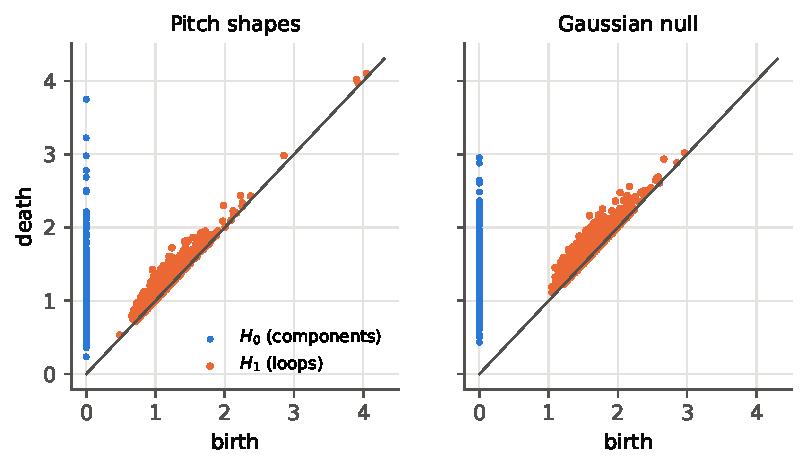
\includegraphics[width=0.7\textwidth]{persistence.pdf}
\caption{Persistence diagrams of 1{,}000 pitch shapes and of a same-covariance Gaussian.}\label{fig:persistence}
\end{figure}

\paragraph{Robustness in flight space.}
The results so far use all nine coordinates, including the delivery and absolute velocity, so we repeated the analyses in flight space (Section~\ref{sec:data}) with the PCA lens, in 2025 and 2026 (Table~\ref{tab:flight}).
The graph is connected at the chosen parameters in both seasons, the gaps and dimension stay below their nulls, and the slow shapes are never isolated, since their separation comes from absolute velocity and delivery and not from the shape of their flight.
The one borderline result is a 2025 loop with persistence \FlMaxPers, just over our cutoff of 2, which 2026 does not repeat.

\begin{table}[htbp]
\centering
\begin{tabular}{lccc}
\toprule
 & Nine features & \multicolumn{2}{c}{Flight space} \\
\cmidrule(lr){3-4}
 & 2025 & 2025 & 2026 \\
\midrule
Components at the chosen parameters & \NComponents & \FlComp & \FlSixComp \\
Slow shapes isolated (\% of fits) & \StabSlowPCALo--\StabSlowPCAHi & \FlSlowIso & \FlSixSlowIso \\
Nerve $b_1$ across the grid & \GridNerveBoneMin--\GridNerveBoneMax{} (\NullNerveBoneMin--\NullNerveBoneMax) & \FlGridNerveMin--\FlGridNerveMax{} (\FlNullNerveMin--\FlNullNerveMax) & \FlSixGridNerveMin--\FlSixGridNerveMax{} (\FlSixNullNerveMin--\FlSixNullNerveMax) \\
Long-lived $H_0$ bars & \PHRealLongBars{} (\PHGaussLongBarsLo--\PHGaussLongBarsHi) & \FlLongBars{} (\FlGaussLongBarsLo--\FlGaussLongBarsHi) & \FlSixLongBars{} (\FlSixGaussLo--\FlSixGaussHi) \\
Largest loop persistence & \PHMaxPers{} (\PHGaussMaxPersLo--\PHGaussMaxPersHi) & \FlMaxPers{} (\FlGaussMaxPersLo--\FlGaussMaxPersHi) & \FlSixMaxPers{} (\FlSixGaussMaxPersLo--\FlSixGaussMaxPersHi) \\
Intrinsic dimension (MLE) & \DimMLE{} of 9 (\DimNullMLE) & \FlDimMLE{} of 6 (\FlDimNullMLE) & \FlSixDim{} of 6 (\FlSixDimNull) \\
\bottomrule
\end{tabular}
\caption{The shape results with all nine coordinates and in flight space, PCA lens. Values in parentheses come from the null models. For nerve $b_1$ they are the range over the Gaussian and within-type-shuffle nulls, for $H_0$ bars and loop persistence the same-covariance Gaussian, and for dimension the spin-pair shuffle. Persistence is measured in units of the median $H_0$ death of the real data, and a loop counts as persistent above 2.}\label{tab:flight}
\end{table}

Pitch-shape space is therefore one connected continuum apart from the very slowest pitches, which join it in flight space at the chosen parameters.
It has no gaps beyond those of a Gaussian, no loop that persists in both seasons, low intrinsic dimension, and, at the level of single pitches, three dense regions.

%======================================================================
\section{Consequences for pitch evaluation}\label{sec:consequences}
%======================================================================
We use our own Stuff+-style models (Section~\ref{sec:grading}). They are gradient-boosted decision trees in CatBoost \parencite{dorogush2018catboost} that predict contact quality (xwOBA), swinging strikes, and chases from release speed, release position, movement, spin rate, spin axis, and extension. We trained them on \StuffTrainN{} pitches from 2022--24 with five-fold out-of-fold predictions, so the 2025 and 2026 seasons are out of sample.
We grade a pitch against its own pitch type. Each component is standardized against the type's reference distribution, the components are combined with equal weights, and the result is rescaled to $100 \pm 15$ within the type.

\subsection{Grading within a label is fragile near boundaries}\label{sec:labelfragile}
If pitch types are regions of a continuous space, a pitch near the edge of its region could be graded very differently depending on which side its label falls, and we wanted to measure how much.
We call a pitch shape with at least 150 pitches a \emph{boundary pitch} if at least half of its 20 nearest shapes from other pitchers carry one other label, with distance measured in flight space. We then grade it twice, once against each label.
In 2025, \LSTwentyFiveBoundary{} of \LSTwentyFiveEligible{} shapes (\LSTwentyFiveBoundaryPct\%) are boundary pitches.
Relabeling moves their grade by a median of \LSTwentyFiveShift{} points. Of the boundary pitches, \LSTwentyFiveOneSDPct\% move by at least one standard deviation, \LSTwentyFiveCrossPct\% switch between above and below average, and \LSTwentyFiveTwoSEPct\% of the shifts exceed twice the grade's own sampling error.
In 2026 the effect replicates, with \LSTwentySixBoundary{} of \LSTwentySixEligible{} boundary pitches, a median shift of \LSTwentySixShift, and \LSTwentySixTwoSEPct\% of shifts beyond twice the sampling error.
To check that this effect does not come only from our model, we also ranked each boundary pitch's actual swinging-strike rate among its own label's pitches and among its neighbor label's pitches. The two percentiles differ by a median of \LSTwentyFivePctChange{} points in 2025 and \LSTwentySixPctChange{} in 2026.
The most common pairs in 2025 are slider and cutter (SL/FC, \LSPairFCSL{} boundary pitches), changeup and splitter (CH/FS, \LSPairCHFS), curveball and knuckle curve (CU/KC, \LSPairCUKC), and slider and sweeper (SL/ST, \LSPairSLST).
While building this test, we found and removed two artifacts. First, a pitcher's own pitches looked close to each other because of their shared delivery, so we use only other pitchers' shapes as neighbors. Second, absolute velocity made hard changeups look like other pitchers' sinkers, so we use relative velocity.
The claim concerns grading \emph{within} a label, as per-type scales and any ``elite among sliders'' comparison do.

%======================================================================
\section{Discussion and conclusions}\label{sec:discussion}
%======================================================================
\subsection{Comparison with prior work}\label{sec:prior}
Several groups have grouped pitches by their physics alone.
\textcite{pane2013trouble} classify PITCHf/x pitches by model-based clustering with a multivariate Gaussian mixture.
\textcite{camp2020clustering} apply $k$-means to the movement, velocity, and spin rate of 2016--17 Statcast pitches and find 30 subtypes within the nine prominent Statcast pitch types for each handedness. These clusters subdivide the existing labels without testing them.
Closest to this paper, \textcite{maloof2026classify} apply persistent homology to a smoothed density of 4.47 million NCAA Division I pitches, in speed relative to the pitcher's fastest pitch, horizontal break, and induced vertical break.
They find three dominant density peaks (fastball, breaking ball, and changeup), draw the boundaries between them by watershed segmentation, and, combining persistent homology with curvature and spectral-graph analyses, conclude that finer pitch names are locations along continuous ridges. Their article is not peer-reviewed.

Our results agree with theirs at the level of density peaks, even though we used Major League data, nine coordinates including spin and release, and one point per pitcher and pitch type.
Our shape results come from different methods, namely Mapper and its nerve, Vietoris--Rips persistence, and null models. The density-peak analysis itself follows theirs (Section~\ref{sec:peaks}).
We did not repeat their curvature and spectral analyses, so their conclusion about ridges is consistent with our picture but not something we tested.
Our null-model results also bear out the concern of \textcite{topaz2026null}. The velocity ordering of the graph and the slider--cutter ``bridge'' are both reproduced by covariance-matched nulls (Section~\ref{sec:shape}), so neither counts as hidden structure.

\subsection{Limitations}\label{sec:limits}
Several limitations should be kept in mind.
The nine-coordinate shape results use one season, although the flight-space check (Table~\ref{tab:flight}) and the evaluation results replicate in 2026.
The fit applies no minimum pitch count. The Mapper features survive minimums of 10 and 20 (Appendix~\ref{app:thin}), but we did not rerun persistent homology and intrinsic dimension with a minimum.
We compare persistence diagrams with null models instead of computing formal confidence sets, and our persistence cutoffs are conventions.
We chose Mapper's parameters by a grid instead of a principled method such as that of \textcite{carrieremicheloudot2018}.
Finally, the Stuff+-style models are our own reimplementation and have not been published.

\subsection{Future studies}
Several natural next steps follow from this work.
Movement could be measured relative to the pitcher's arm slot, which would mean redesigning the features and not just adding a column.
Delivery and biomechanical markers, such as pronation and supination, are not recorded by Statcast and are left for future work.
The analysis could be repeated in other seasons and at other levels, and Mapper's parameters could be chosen by a principled method.
Pitch development is a natural next question. Exploratory tests designed in advance suggest that drifting toward better-scoring neighbors does not predict next-season gains, while more typical shapes get fewer whiffs than their physics predicts, and a planner that routes a pitch through shapes other pitchers already throw could be built on these results and tested prospectively.

\subsection{Conclusion}\label{sec:conclusion}
Mapper gives a readable picture of pitch-shape space, and homology, null models, dimension estimates, and density peaks tell us which parts of that picture hold up.
The space is one connected continuum apart from the very slowest pitches, with no gaps beyond a Gaussian, no loop that persists in both seasons, low intrinsic dimension, and three dense regions at the level of single pitches.
The finer pitch labels divide this continuum, and they do not mark separate clumps.
This has a practical consequence. Grading a pitch within its label is fragile for pitches near a boundary, so a pitch is better described by where it sits in shape space as well as by its tag.

%======================================================================
\section{Acknowledgments}
%======================================================================
\plan{Will to write: thank the advisor, committee, and anyone else who helped.}

\appendix
\section{Parameters and reproducibility}\label{app:repro}
\begin{table}[htbp]
\centering
\begin{tabular}{ll}
\toprule
Component & Setting \\
\midrule
Lens & PCA, 2 components (alternatives: velocity $\times$ IVB, Isomap, density) \\
Cover & 10 intervals per axis, 30\% overlap (grid: 8/10/12, 20/30/40\%) \\
Clustering & DBSCAN, $\varepsilon = 1.0$, $M = 4$ (grid: $\varepsilon$ = 0.8/1.0/1.2) \\
Stability & 30 refits on 80\% of pitchers without replacement \\
Null models & Gaussian; within-type shuffle; spin-pair shuffle \\
Persistent homology & Vietoris--Rips, five 1{,}000-shape subsamples \\
Intrinsic dimension & MLE with 10 neighbors; TwoNN \\
Density peaks & $50^3$ grid, $\sigma = 1$ cell, 50 Gaussian replicates \\
\bottomrule
\end{tabular}
\caption{Parameters.}
\end{table}
Code and data products are at \url{https://github.com/WillPaz16/tda-pitch-clustering}. Every number in this paper is generated from saved outputs by \texttt{src/viz/paper\_numbers.py}, and every figure by \texttt{src/viz/thesis\_figures.py}. The running example is computed by \texttt{src/tda/circle\_example.py}.

\section{Minimum pitch counts}\label{app:thin}
Table~\ref{tab:thin} repeats the main Mapper fit with a minimum number of pitches per shape.
The velocity ordering is unaffected. Slow shapes stay off the continuum, but at a minimum of 20 they are too few to form clusters of their own.

\begin{table}[htbp]
\centering
\begin{tabular}{rrrrcc}
\toprule
Minimum pitches & Shapes & Slow shapes & Components & Slow shapes isolated & Velocity ordering $\rho$ \\
\midrule
1 & \SSOneShapes & \SSOneSlow & \SSOneComp & \SSOneIso & \SSOneRho \\
10 & \SSTenShapes & \SSTenSlow & \SSTenComp & \SSTenIso & \SSTenRho \\
20 & \SSTwentyShapes & \SSTwentySlow & \SSTwentyComp & \SSTwentyIso & \SSTwentyRho \\
\bottomrule
\end{tabular}
\caption{The main Mapper fit with a minimum pitch count per shape.}\label{tab:thin}
\end{table}

\section{Use of AI assistance}
This project was developed with substantial help from Claude, Anthropic's AI assistant, used through Claude Code, which assisted with analysis code, documentation, the literature search, and drafting.
The author set the research questions and scope, made the methodological decisions, and reviewed the results.
Because AI output can be confidently wrong, the work was built around verification. Every structural claim is tested against null models and across parameters, subsamples, and lenses before it counts as a finding, and several early findings were dropped this way. A citation is used only after its bibliographic data match a registry record and the claim is confirmed at a specific page of the source, with an independent check and the author's review.

\printbibliography

\end{document}
